\section{Thesis Overview}

Magnetic resonance imaging (MRI) provides an excellent modality for distinguishing different tissues 
in the human body, which makes 
this modality essential for medical applications. MRI can also be used for treatment planning of 
medical procedures that require a great degree of geometrical accuracy such as  
functional radiosurgery~\cite{Kond99}. Unfortunately, the accuracy of MRI for medical targeting applications 
is compromised by the presence of geometric distortions such as non-linearities of the magnetic gradient 
fields or inhomogeneities of the scanner main field 
~\cite{Dor05,LSS06a,LSS06b,LSS08a,LSS08b,Lang99,Wang04a,Wang04b}. 
Gradient nonlinearities can cause over 2mm of distortion to the location of features in the 
image~\cite{LSS08b,Lang99}.

% Modern MRI scanners have built-in distortion correction algorithms, that rely on knowledge of the magnetic 
% field configuration and its distortion. Built-in algorithms, which are usually proprietary, are designed 
% based on assumed knowledge of the geometry and location of the gradient coils. A more practical approach is 
% to use a phantom of known geometry and to derive the distortion by analyzing the MRI images generated with 
% such a phantom ~\cite{Dor05,LSS06a,LSS06b,LSS08a,LSS08b,Lang99,Wang04a,Wang04b}. 
% This method has the advantage that a scanner-specific correction can be applied, which can also take into 
% account potential changes in the gradient fields over time.

% Accurate knowledge of the gradient isocenter is essential to very accurate distortion correction methods, 
% To our knowledge, existing distortion correction algorithms, both built-in and phantom based, 
% make the assumption that the gradient isocenter coincides with the origin of the DICOM coordinates. 
% This assumption may not be accurate and should not be used if a high degree of accuracy is necessary.

% The goal of this work was to develop and implement a numerical software-based method to estimate the gradient 
% isocenter of the magnetic field inside an MRI scanner using the MRI scan of a custom-built phantom.  
% In our previous work~\cite{LSS06a,LSS06b,LSS08a,LSS08b}, we used an oil filled plexiglas cube with
% 159.50mm $\times$ 159.70mm $\times$ 158.11mm dimension that was designed to fit MR scanners that were 
% available at that time.  Current MRI scanners have a significantly wider aperture, which necessitates 
% a larger phantom to characterize the field distortion.  Furthermore, since the lower part of the scanner 
% aperture is occupied by the scanner table, the scanning area occupied by the phantom or the patient is not 
% centered on the gradient isocenter, making correction methods that assume that the phantom is centered with 
% respect to the gradient isocenter~\cite{LSS06a,LSS06b,LSS08a,LSS08b,Lang99} obsolete and potentially 
% inaccurate.

% \begin{figure}[htb]
%   \begin{minipage}{0.80\linewidth}
%     \centering
%     \centerline{\mbox{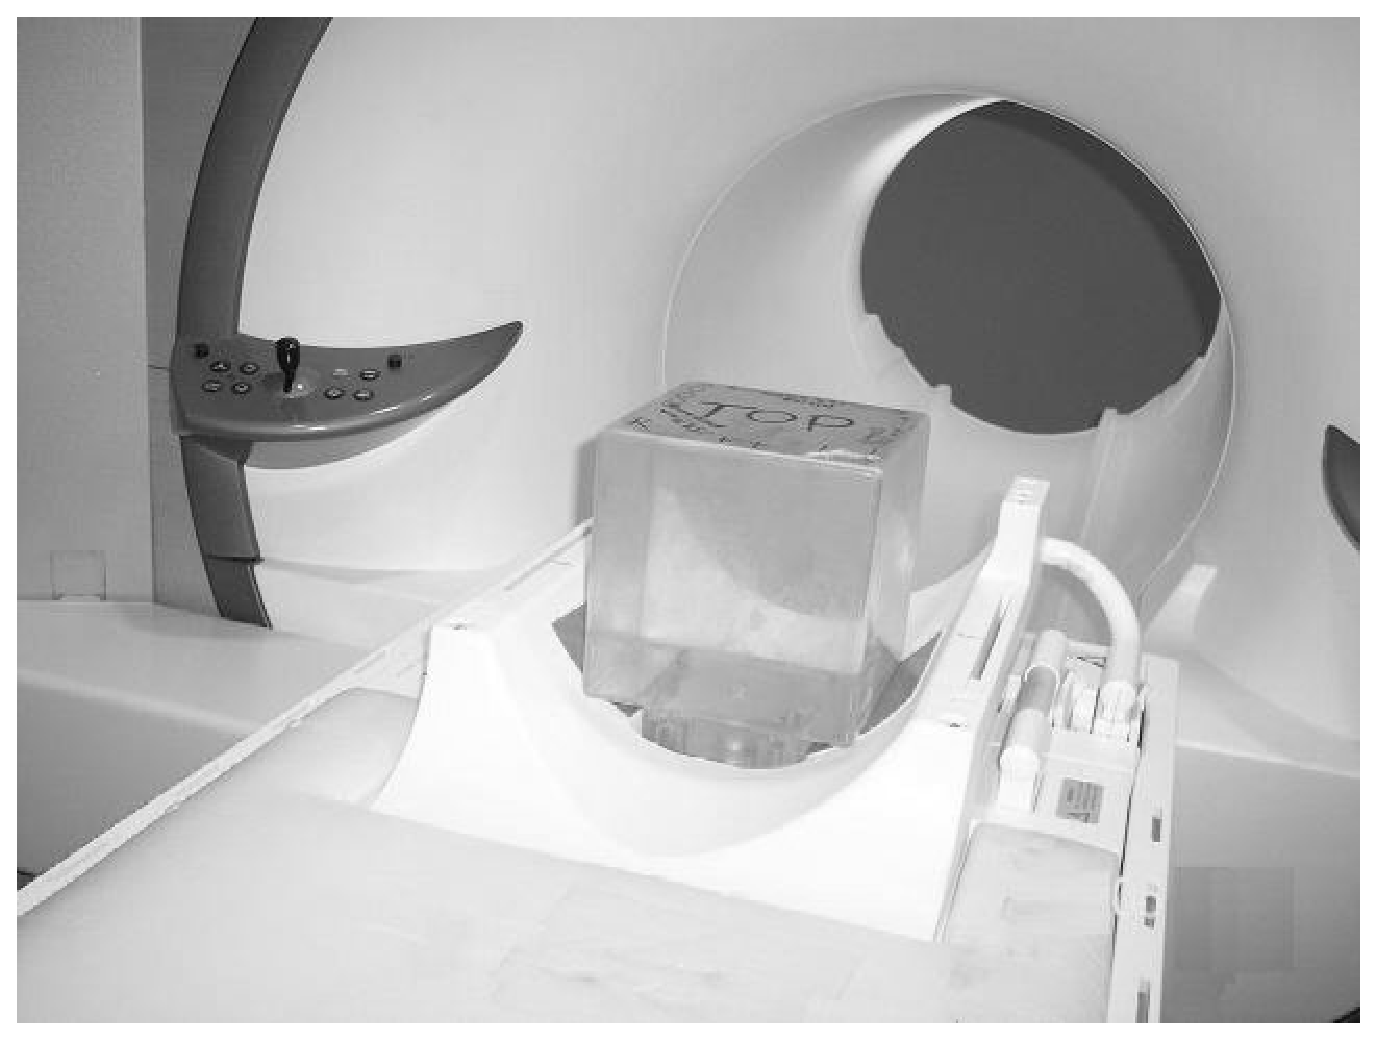
\includegraphics[width=4in]{introduction/images/phantom_scanner2.eps}}}
% %    \centerline{New device}\medskip
%     \centerline{}\medskip
%   \end{minipage}
%   \caption{A phantom cube made of plexiglas and filled with oil is ready for scanning} \label{fig:1}
% \end{figure} 

The primary purpose of this thesis was to improve the distortion correction method developed in a previous 
thesis.  To do this, the following issues were addressed in this work:
\begin{itemize}
\item A new phantom was designed that can capture the distortion in modern 3-Tesla(T) MRI scanner. 
\item Algorithms were developed that can extract relevant data points from the MR images of the new phantom.
\item An new algorithm was developed that can accurately estimate the gradient isocenter of the magnetic 
  field inside 3T MRI scanners.
\item An algorithm was developed that can determine the undistortion paramters, which can then be used to 
  generate undistorted MR images.
% \item An algorithm was developed that can accurately estimate the undistortion paramters,
%   which could then be used to generate undistorted MR images.
\end{itemize}

% background 
The thesis is organized as follows. After the introduction, Chapter 2 gives background information on MRI, 
it's geometric distortion, and approaches to corrected. 
Chapter 3 describe the design details of the new phantom and several phases and changes the design 
went through. The main feature of the final design of the phantom and their importance will be discussed.
The next chapter discusses the algorithm for estimation of  gradient isocenter based on new
phantom design. % Since there is no way to know the accurate location of isocenter inside MRI scanner, not even
% the manufacture themselves, we will analyze our result using a simulate data points. 
Chapter 5 describe a series of algorithms used to extract relevant data from MR and CT images. CT images were
used in this work to obtain accurate dimensions inside the phantom.
% After isocenter algorithm we will start to discuss a series of algorithms we used to extract data points
% from MR images and CT images. CT images is used for measuring certain dimensions inside phantom due to
% limitations of manufacture's macine. 
Chapter 6 describes the procedure to estimate the parameters of the model that undistorts the distorted 
MR images. The final chapter summarizes the main results and suggests future work.
% In the final chapter, putting everything together, 
% we are using the geometric feature of the phantom and information
% obtained from MR images to estimating a undistortion parameter that can transform the distorted MR images
% back to undistorted images.

\section{Background}

The clinical application of protons was first suggested over 60 years ago \cite{Wil46}.
The ability to penetrate human tissue, delivering high dosage of proton beams at a target
region and being able to concentrate on a very small target area make protons ideal for use in noninvasive surgery \cite{Wil46}. Currently, Loma Linda University
Medical Center (LLUMC) is using proton beams to treat patients with tumors or
vascular malformations in the brain.
Due to the effectiveness of proton radiosurgery, a new system is proposed to treat
even smaller targets, more specifically, cranial targets.  However, this requires higher
accuracy of the treatment system. The current system can treat targets as small as 1 to 3 cm.  Target localization is accomplished using CT and projection angiography.
In order to achieve higher accuracy, MRI is to be used for target localization in the new
system. The major obstacle of using MRI is the gradient nonlinear
distortion on MRI images caused by the magnetic field of the scanner.
Two of the most important requirements for a successful distortion correction are:

\begin{enumerate}
\item The distortion correction must have submillimeter accuracy.
\item The correction process must be finished within 15 minutes.
\end{enumerate}

% I added some more detail in this paragraph

%The iteracy that this work is based on presented gradient nonlinearity correction method based on a cubic phantom MRI data set\cite{tom}.
This work is based on a published method for gradient nonlinearity correction using a cubic phantom MRI data set \cite{tom}. The published method utilizes the sum of spherical
harmonics to model the geometrically warped planes of the cube, and applies the model
to correct arbitrary image sets acquired with the same scanner. The cube is
placed in the MRI scanner such that the cube's center is exactly in the center of the MRI scanner.  This work assumes the center of the MRI scanner corresponds to the isocenter of the
magnetic field of the scanner. Opposite faces of the phantom are averaged, and three midplanes are fit to these surfaces.  Due to the symmetric property of the magnetic field,
the midplanes of different orientations of the phantom cube are undistorted.  Through each midplane, the ideal planes of different surfaces
of the cube are calculated simply by shifting the midplane to the direction
of the ideal plane by one-half the length of the cube. For each pixel on
the ideal plane, the sum of spherical
harmonics equation \ref{eq:spherical_harmonics} is applied to transform that pixel to the corresponding location on the distorted plane.

\begin{equation} \label{eq:spherical_harmonics}
\bar{\alpha} = \alpha(1 + K_{\alpha_0}(x^2 + y^2) + K_{\alpha_1}z^2 +
K_{\alpha_2}z^2(x^2 + y^2) + K_{\alpha_3}(x^2 + y^2)^2 +
K_{\alpha_4}z^4)
\end{equation}

Where $\bar{\alpha}$ and $\alpha$ are undistorted and distorted 3D coordinate respectively; $x$, $y$ and $z$ are coordinates of $\alpha$ on each axis; $K_{\alpha_i}$ are distortion parameters. Thus the distortion parameters in
equation \ref{eq:spherical_harmonics} are computed using linear least squares
technique.

Several assumptions are made for this model:
\begin{itemize}
  \item The phantom is (reasonably) centered with respect to the gradient isocenter of the scanner.
  \item The distortion is (reasonably) symmetric for each pair of faces.
  \item The origin of the DICOM patient coordinate system represents the position of the gradient isocenter.
\end{itemize}

However, positioning the phantom with respect to gradient isocenter is very difficult,
making it nearly impossible to perfectly center the phantom. After performing numerous
scans by Permedics Inc and LLUMC over the past several years, the issue of phantom centering has been identified
as a crucial factor in the quality of image data.  Improper centering of the phantom
in the scanner produces strong asymmetry in the phantom surfaces, thereby affecting the
accuracy of the distortion correction.  Therefore, the assumption that the distortion
is symmetric for each pair of phantom faces is invalid.

The assumption that the origin of the DICOM patient coordinate system corresponds to the isocenter of the magnetic field in the MRI scanner is also invalid. Siemens
engineers have confirmed that the true location of the gradient isocenter is unknown.
Investigating this further appeared to confirm this claim:  every scan performed thus far features a -10mm offset in Y in order to center the field of view on the phantom.  Therefore, the DICOM origin is shifted -10mm in $Y$ for each image.  But, the distortion inherent to each pair of phantom surfaces appears to be quite symmetric.  If the gradient isocenter was truly located at the DICOM origin, then the images would be expected to contain significant asymmetry in the distortion.  This is not the case in recent phantom studies.

In addition, the computation, including image filtering, distortion parameters
computation and final correction, average takes about 20-30 minutes.  In some cases, the calculation
could require as much as 40 minutes. This is far from the ideal 15 minutes requirement for clinical use.

\section{Significance}

% Which equation are you referring to here?  It would be better to reference the equation, instead of saying "the equation above"

Consider the minimization of the original expression for the sum of spherical harmonics:

\begin{equation} \label{eq:spherical_harmonics_2}
0 = \alpha(1 + K_{\alpha_0}(x^2_i + y^2_i) + K_{\alpha_1}z^2_i +
K_{\alpha_2}z^2_i(x^2_i + y^2_i) + K_{\alpha_3}(x^2_i + y^2_i)^2 +
K_{\alpha_4}z^4_i)
\end{equation}

The correction method this work proposes is on a pixel-to-pixel basis instead of a plane to plane basis.
Consider a point $P$ = $[X,Y,Z]$, where $X$, $Y$, and $Z$ are represented in equation \ref{eq:spherical_harmonics_2}. Each $X$, $Y$, and $Z$ describes the distance of $P$ from the DICOM origin (gradient isocenter), previously assumed to be at [0,0,0].  Past MRI studies have confirmed that the gradient isocenter is not at [0,0,0], therefore it is necessary to shift the DICOM origin appropriately by some offset $[\delta,\beta,\gamma]$.  Shifting the DICOM origin by this amount yields the new expression for $P$:

\begin{eqnarray}
P = [X - \delta, Y - \beta, Z - \gamma]
\end{eqnarray}

Substitute the new expression for $P$ into the sum of spherical harmonics expression:

$$0 = \alpha(1 + K_{\alpha_0}((x_i - \delta)^2 + (y_i - \beta)^2)$$
$$+ K_{\alpha_1}(z_i - \gamma)^2 + K_{\alpha_2}(z_i - \gamma)^2((x_i - \delta)^2 + (y_i - \beta)^2)$$
$$+ K_{\alpha_3}((x_i - \delta)^2 + (y_i - \beta)^2)^2 + K_{\alpha_4}(z_i - \gamma)^4)$$

Therefore, by expressing $P$ in this manner, the position of the true gradient isocenter becomes
$[\delta, \beta, \gamma]$. To solve for $\delta$, $\beta$, $\gamma$ and $K_{\alpha}$, we do not need
to have a full plane, as long as enough data points exist, and each data point exhibits a significant amount of distortion. The system can be solved using a linear least squares technique.

% To collect the data sets, a new phantom (Fig \ref{fig:2}), is proposed to capture data points on only the corner sections
% of the original phantom cube.  Since these sections are located far away from the gradient isocenter, they will exhibit the largest amount
% of distortion when compared to other sections closer to the gradient isocenter. The image slices that
% would be used are those close to each surface of the phantom. For each of these images a 
% filtering process will be applied to obtain only data points on the edge of phantom cube. 

% \begin{figure}[htb]
%   \begin{minipage}{0.80\linewidth}
%     \centering
%     \centerline{\mbox{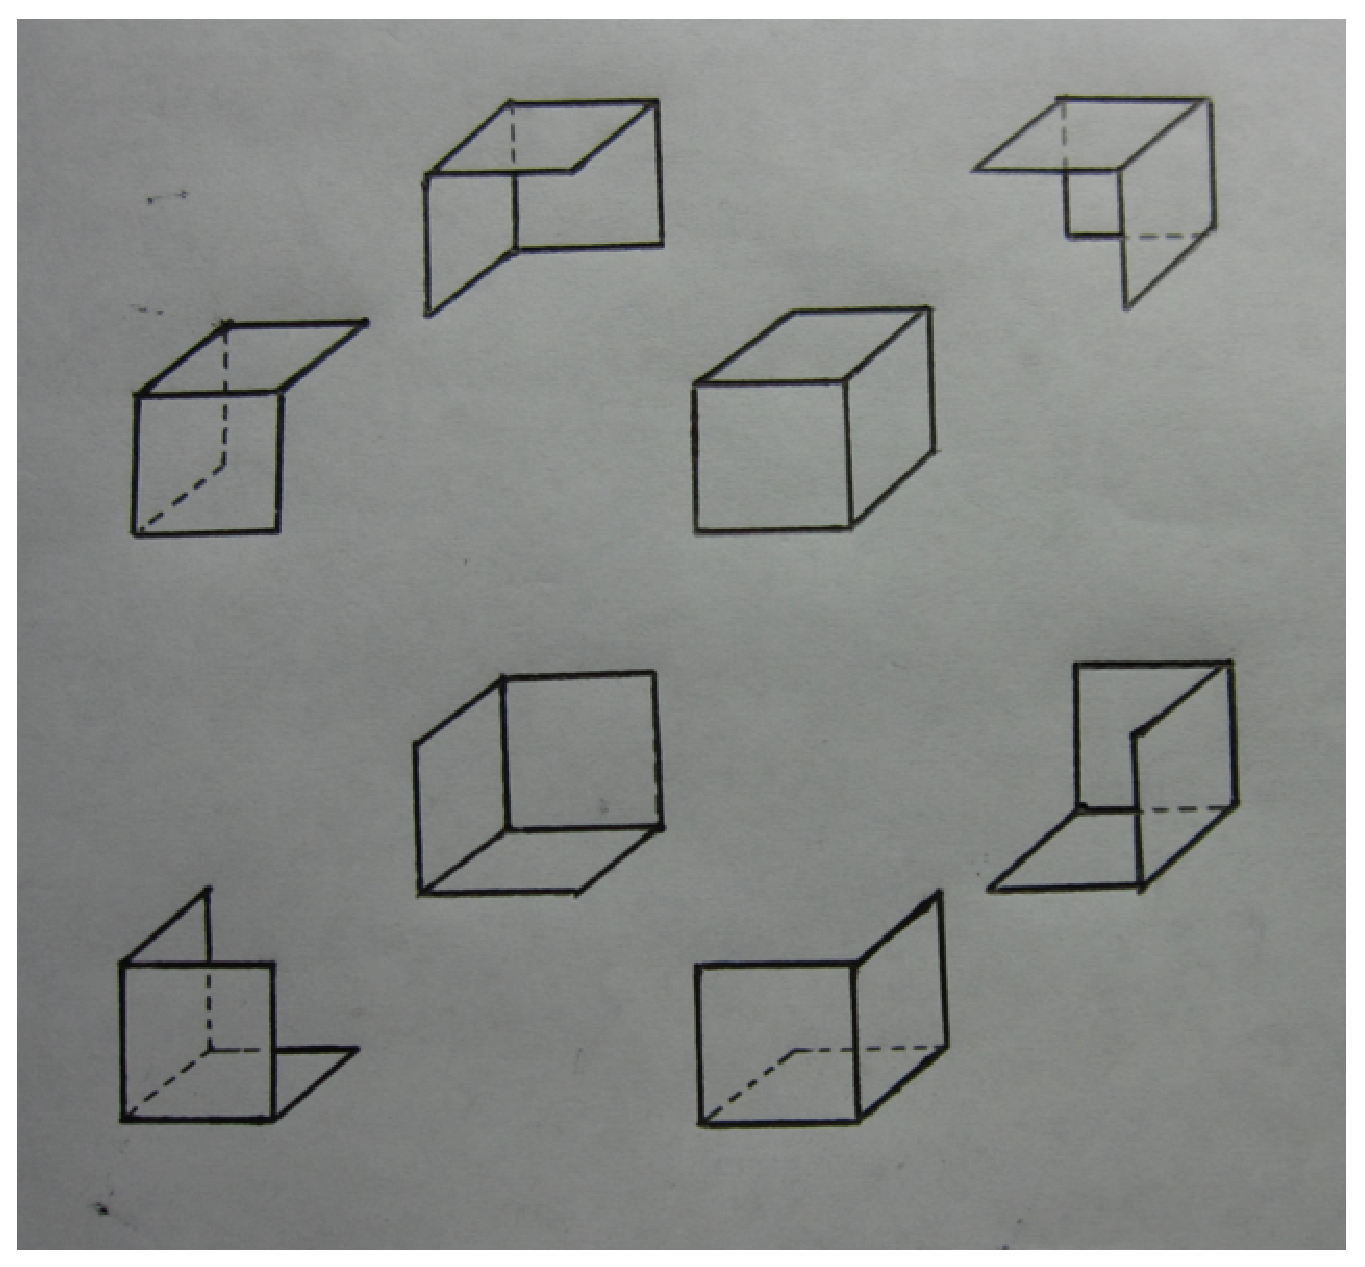
\includegraphics[width=4in]{images/model2.eps}}}
% %    \centerline{New device}\medskip
%     \centerline{}\medskip
%   \end{minipage}
%   \caption{The new phantom, designed to collect data at the corners of the MRI scan.}  \label{fig:2}
% \end{figure}

% The reason for constructing a new phantom is that a phantom cube larger than original size (159.50 mm x 159.70 mm x 158.11 mm) is needed to 
% capture the distortion of larger MRI scanner while the manufacturer who produced the original
% phantom cube was having difficulty produce an accurate cubic phantom larger than the
% one shown in \ref{fig:1}. The eight parts, shown in fig \ref{fig:2}, will be interconnected and placed inside a water tank for scanning.
% For each image, eight curves representing the intersection between the surface of the material
% and water will be obtained, and will be used for calculating the gradient nonlinearity distortion correction.
